\chapter{Descriptive statistics}
\label{app:descriptives}

\FloatBarrier
\section{Gender}

\begin{figure}[htbp]
    \centering
    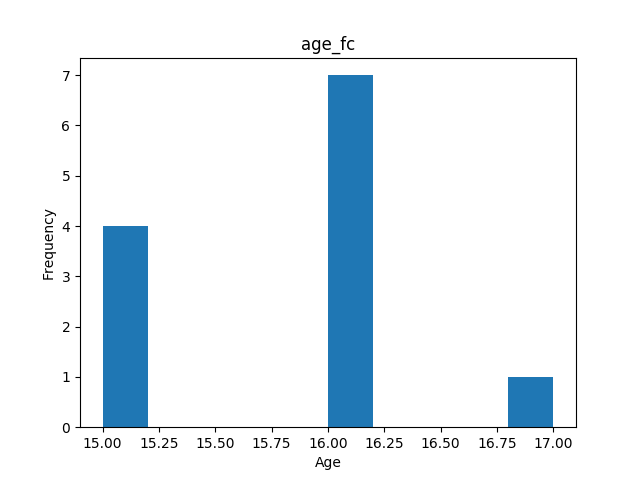
\includegraphics[width=.7\textwidth]{img/age_fc.png}
    \caption{A histogram of the age of the flashcard users finishing the experiment}
\end{figure}
\begin{figure}[htbp]
    \centering
    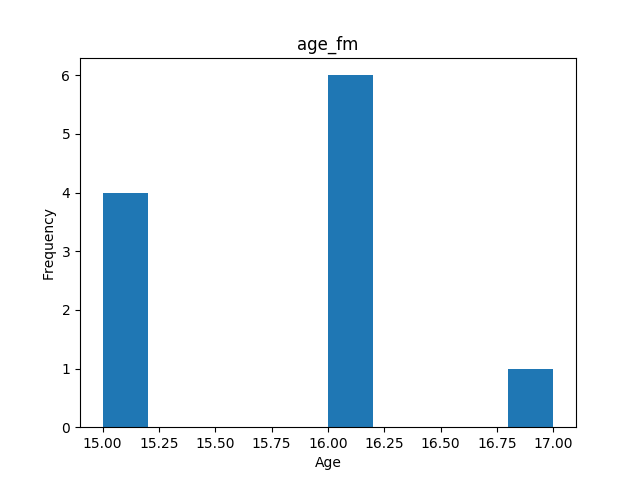
\includegraphics[width=.7\textwidth]{img/age_fm.png}
    \caption{A histogram of the age of the flashmap users finishing the experiment}
\end{figure}
\begin{figure}[htbp]
    \centering
    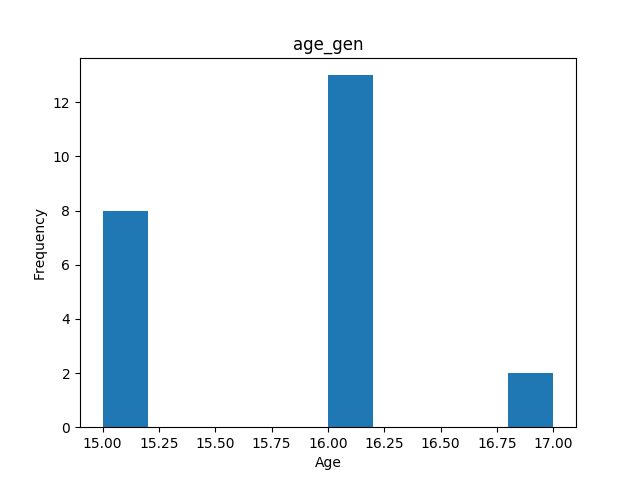
\includegraphics[width=.7\textwidth]{img/age_gen.png}
    \caption{A histogram of the age of all users finishing the experiment}
\end{figure}

\FloatBarrier
\section{Comparisons of ages among conditions}

\FloatBarrier
\subsubsection{Age}

\begin{longtable}[c]{@{}lrrrr@{}}
\toprule\addlinespace
& \textbf{Mann-Whitney-U k} & \textbf{Mann-Whitney-U p} &
\textbf{Welch's t-test k} & \textbf{Welch's t-test p}
\\\addlinespace
\midrule\endhead
& 0.086 & 0.9323 & 0.086 & 0.9325
\\\addlinespace
\bottomrule
    \label{tab:age_comp}
\end{longtable}

\begin{figure}[htbp]
    \centering
    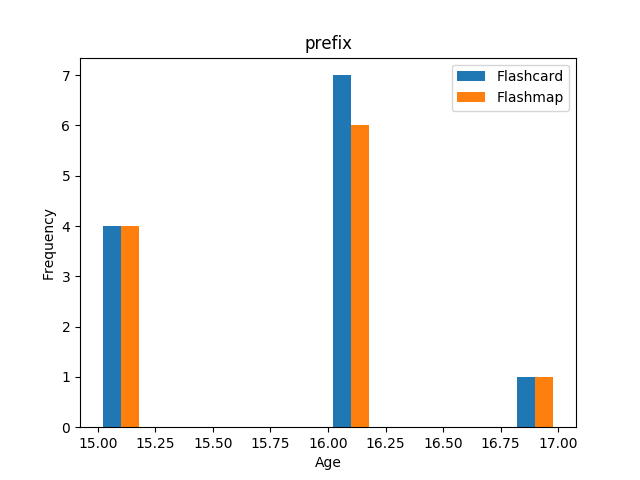
\includegraphics[width=.7\textwidth]{img/age.png}
    \caption{Age comparisons of flashcard and flashmap users}
    \label{fig:age}
\end{figure}
